% !TeX spellcheck = es_ES
% Chapter 1

%\chapter{Chapter Title Here} % Main chapter title
%
%\label{Chapter1} % For referencing the chapter elsewhere, use \ref{Chapter1} 

%----------------------------------------------------------------------------------------

% Define some commands to keep the formatting separated from the content 
%\newcommand{\keyword}[1]{\textit{#1}}
%\newcommand{\tabhead}[1]{\textbf{#1}}
%\newcommand{\code}[1]{\texttt{#1}}
%\newcommand{\file}[1]{\texttt{\bfseries#1}}
%\newcommand{\option}[1]{\texttt{\itshape#1}}

%----------------------------------------------------------------------------------------

\chapter{Calibración Eléctrica}
	Con el objetivo de asegurar que la información registrada por el calorímetro corresponde con un valor específico de potencia, es necesario realizar una calibración eléctrica, la cual es específica para cada canal de medición. Para ello, el equipo cuenta con una resistencia de precisión que envuelve el contenedor de la celda y permite simular, lo mejor posible, la energía liberada en forma de calor cuando una reacción química tiene lugar en la celda, la ubicación de esta resistencia se muestra en la \autoref{fig: resistencia} \cite{Suurkuusk}. 
	\begin{figure}[h]
		\centering
		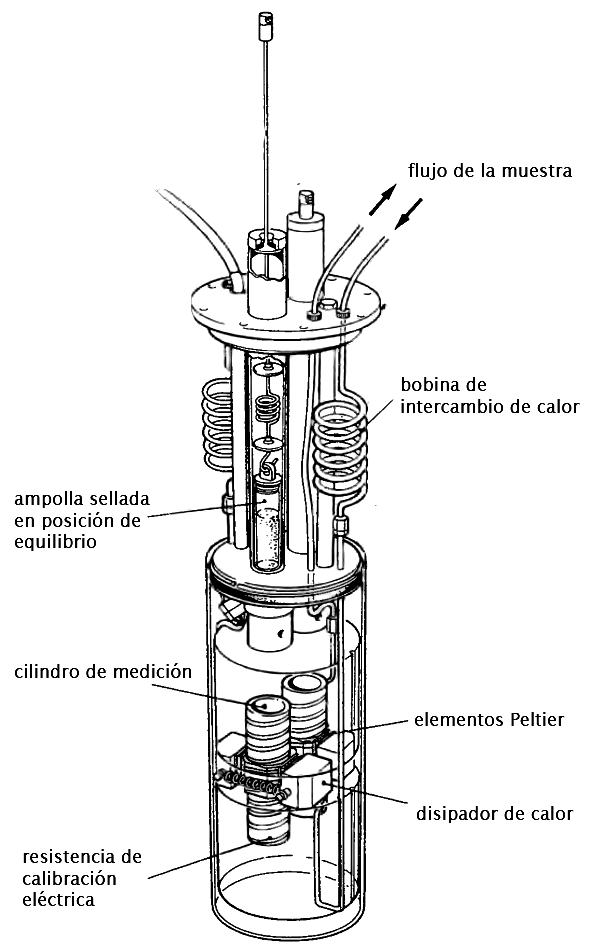
\includegraphics[width=0.45\linewidth]{Figures/resistencia}
		\caption{Interior del cilindro de medición, modificidado de \cite{Suurkuusk}.}
		\label{fig: resistencia}
	\end{figure}
	
	Para calibrar el sistema se realizan lecturas consecutivas de la línea base, esto es la potencia que registra el calorímetro es ausencia de perturbación, y a partir de esto se ajusta el cero del canal, pues se busca que la línea base sea lo más cercana a 0 $\mu$W. Posteriormente, se aplica una potencia conocida sobre la resistencia y hacen lecturas de la potencia registrada por el calorímetro, a partir de esto se ajusta la ganancia, hasta que la potencia aplicada y la registrada tengan el valor más cercano posible. La potencia conocida debe concordar con el valor de amplificación del selector \texttt{RANGE} en la \autoref{fig: controlCal}.
	\begin{figure}[h]
		\centering
		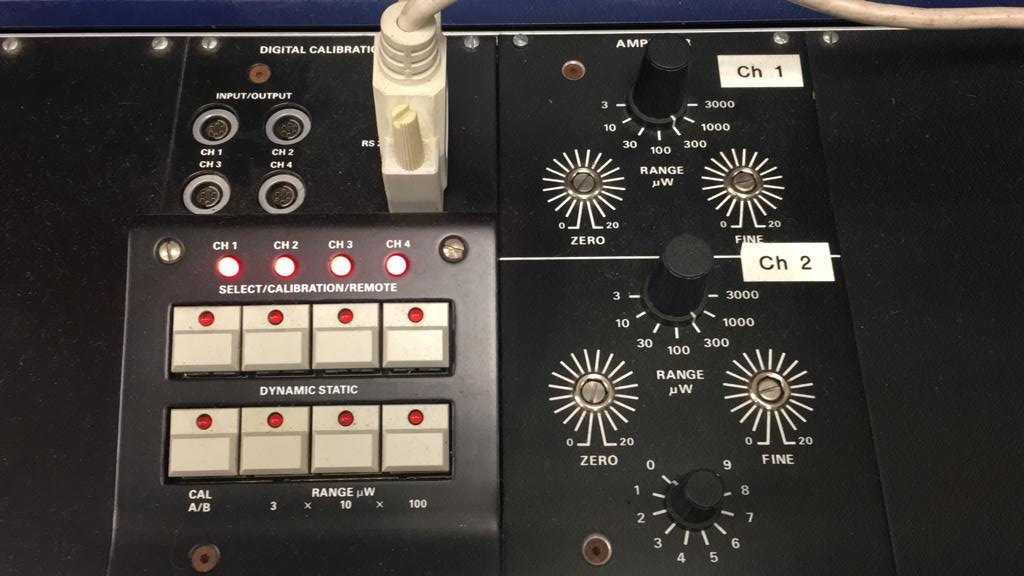
\includegraphics[width=0.7\linewidth]{Figures/controlCal}
		\caption{Control del cero y la ganancia del calor\'imetro}
		\label{fig: controlCal}
	\end{figure}
	
	Existen dos tipos de calibraciones, en la primera se modifican los valores de cero y ganancia en el equipo directamente, mientras que en la segunda los valores corresponden a ajustes en el software. Estos métodos de calibración reciben el nombre de estática y dinámica correspondientemente, y se debe asegurar que al momento de realizar una calibración dinámica, una calibración estática haya sido realizada previamente, pues los valores registrados por software son digitales (discretos), entonces la resolución de estos será determinada por la ganancia del circuito análogo, lo cual sólo es posible de controlar en el calorímetro directamente.
	 
	\section{Est\'atica}
	En la calibración estática, se debe manipular el equipo directamente. En primer lugar como fue mencionado anteriormente se ajusta el cero del canal en ausencia de perturbaciones. Para esto se manipula el potenciómetro de diez vueltas del lado izquierdo el cual está marcado como \texttt{ZERO} en la \autoref{fig: controlCal}, girando en sentido horario el valor de potencia registrado será cada vez menor. Una vez el cero ha sido ajustado, se aplica sobre la resistencia una potencia conocida, por un tiempo determinado por el usuario, y se espera que la señal registrada por el calorímetro en su estado estacionario coincida con el valor aplicado de potencia. Para esto se debe esperar cerca de 20 minutos para que la resistencia alcance el estado estacionario y posteriormente se manipula el potenciómetro derecho (\texttt{FINE} en la \autoref{fig: controlCal}), donde giros en el sentido horario disminuyen el valor de potencia registrado por el equipo, de esta forma se configura la ganancia del equipo.

	Para activar la resistencia es posible hacerlo manualmente a través de los botones blancos que se observan en la \autoref{fig: controlCal}. En primer lugar se selecciona el canal sobre el cual se quiere realizar la calibración, para esto se oprime el botón correspondiente a cada canal (canal 1, botón izquierdo) del panel \texttt{SELECT}, esto ocasionará que la luz asociada a ese canal comience a oscilar. Posteriormente, si la luz continúa en este estado se debe volver a presionar el botón de \texttt{SELECT} asociado a este canal. El lado de la calibración A ó B se selecciona oprimiendo el botón \texttt{CAL A/B} donde la luz prendida indica A, y la potencia oprimiendo los botones de \texttt{RANGE} cuyo producto da el valor de potencia deseado en $\mu$W. Finalmente, para activar la calibración se oprimen de manera simultánea el botón de \texttt{SELECT} del canal y el botón \texttt{CAL A/B}. Una vez se haya calibrado el estado estacionario, la resistencia se apaga oprimiendo el botón del canal en \texttt{SELECT} y posteriormente, al mismo tiempo este botón y \texttt{CAL A/B}.
	
	Otra manera de hacerlo es a través del software Digitam. En donde se realiza un método experimental que contenga la calibración eléctrica, este método ya se encuentra creado bajo el nombre \texttt{staticCalibration.tam}, el cual:
	\begin{itemize}
		\item Mide por 30 minutos la línea base.
		\item Aplica 300 $\mu$W sobre el lado B del canal 1 (referencia) por 35 minutos.
		\item Espera por 45 minutos a que la potencia se estabilice en la línea base.
	\end{itemize}

	Resultados de calibraciones estáticas se muestran en la \autoref{fig: staticCalibrations}. En particular, para el caso de la \autoref{fig: noAmpCal} se tiene que el cero está bien ajustado, sin embargo el valor de la amplitud no corresponde, pues el sensor se satura a un valor de 213,9 $\mu$W, sin una transición suave al estado estacionario. El efecto contrario se observa en la \autoref{fig: noZeroCal}, pues la potencia aplicada corresponde con la leída, sin embargo, la línea base se encuentra a -80,1 $\mu$W.
	\begin{figure}[h]
		\centering
		\begin{subfigure}{0.45\linewidth}
			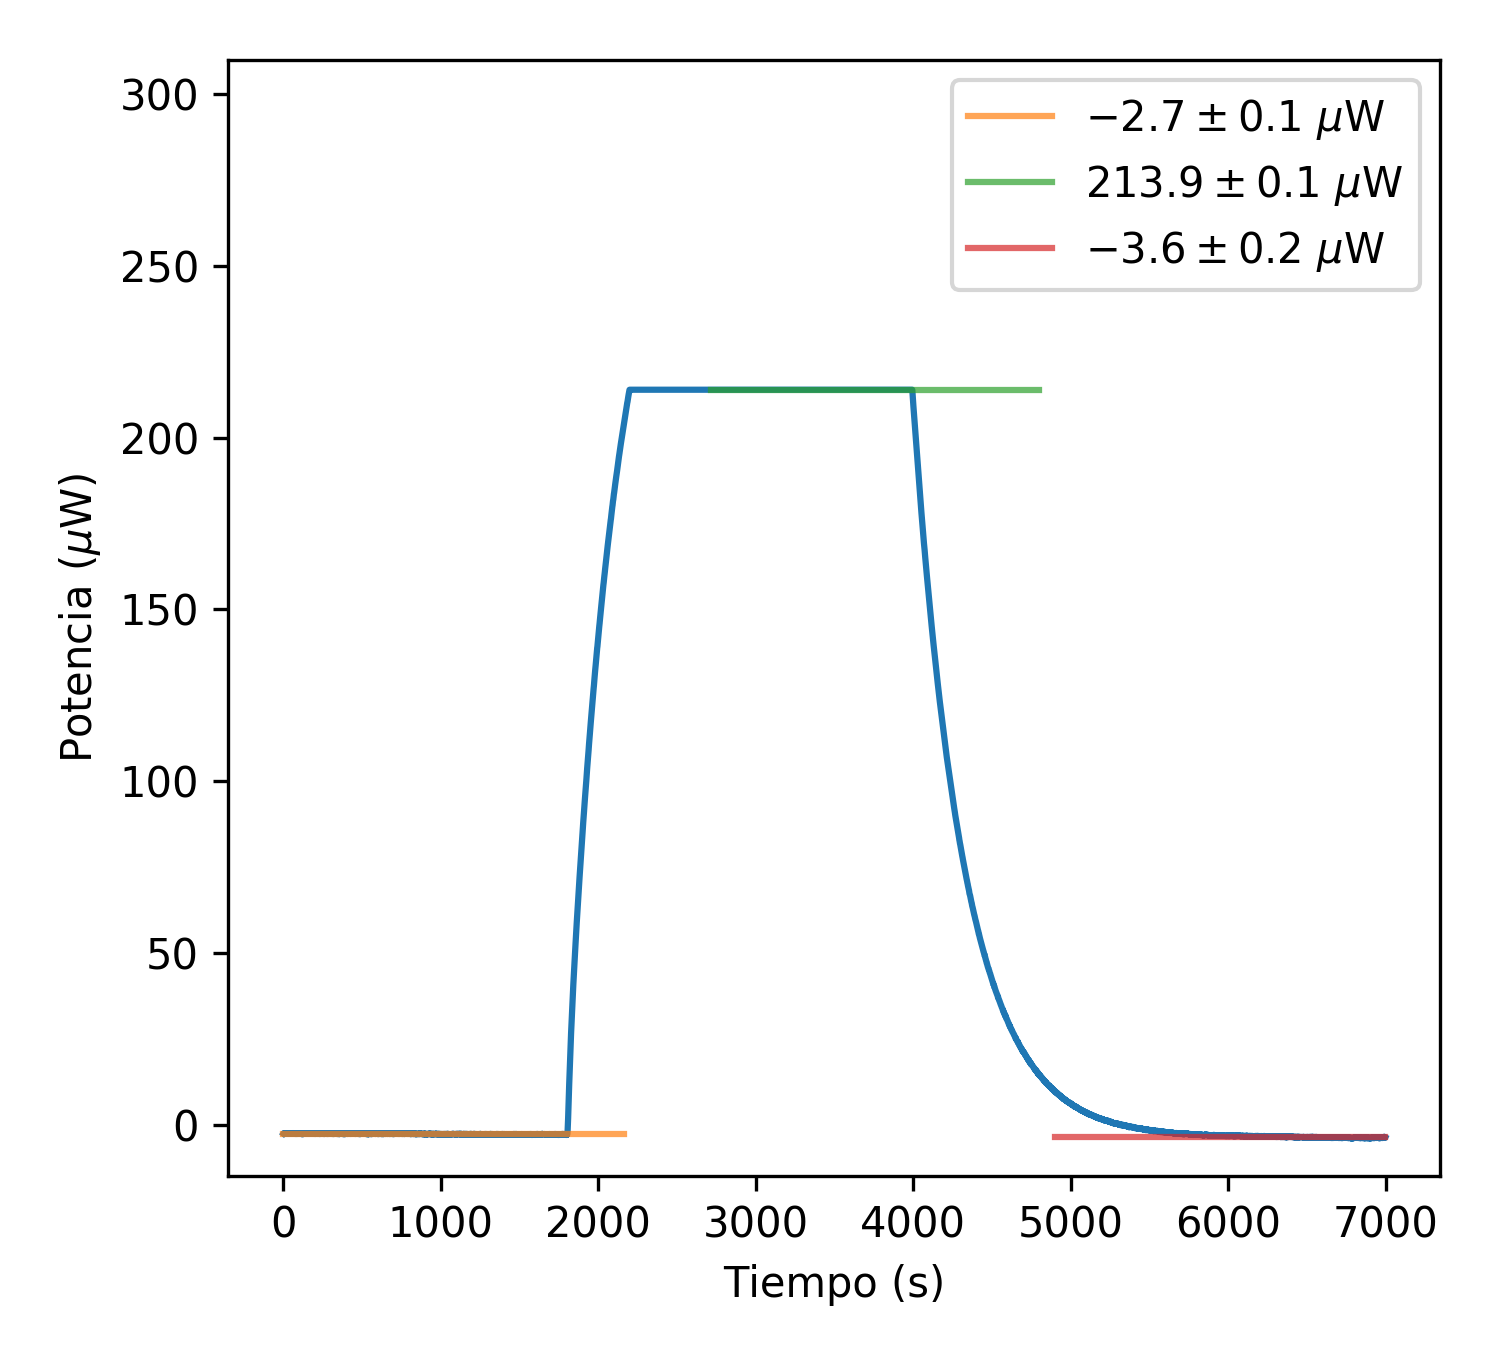
\includegraphics[width=\linewidth]{../Data/ElectricalCalibrations/Static/Calibration1}
			\caption{Potencia medida: $216.6 \pm 0.2$ $\mu$W.}
			\label{fig: noAmpCal}
		\end{subfigure}
		\begin{subfigure}{0.45\linewidth}
			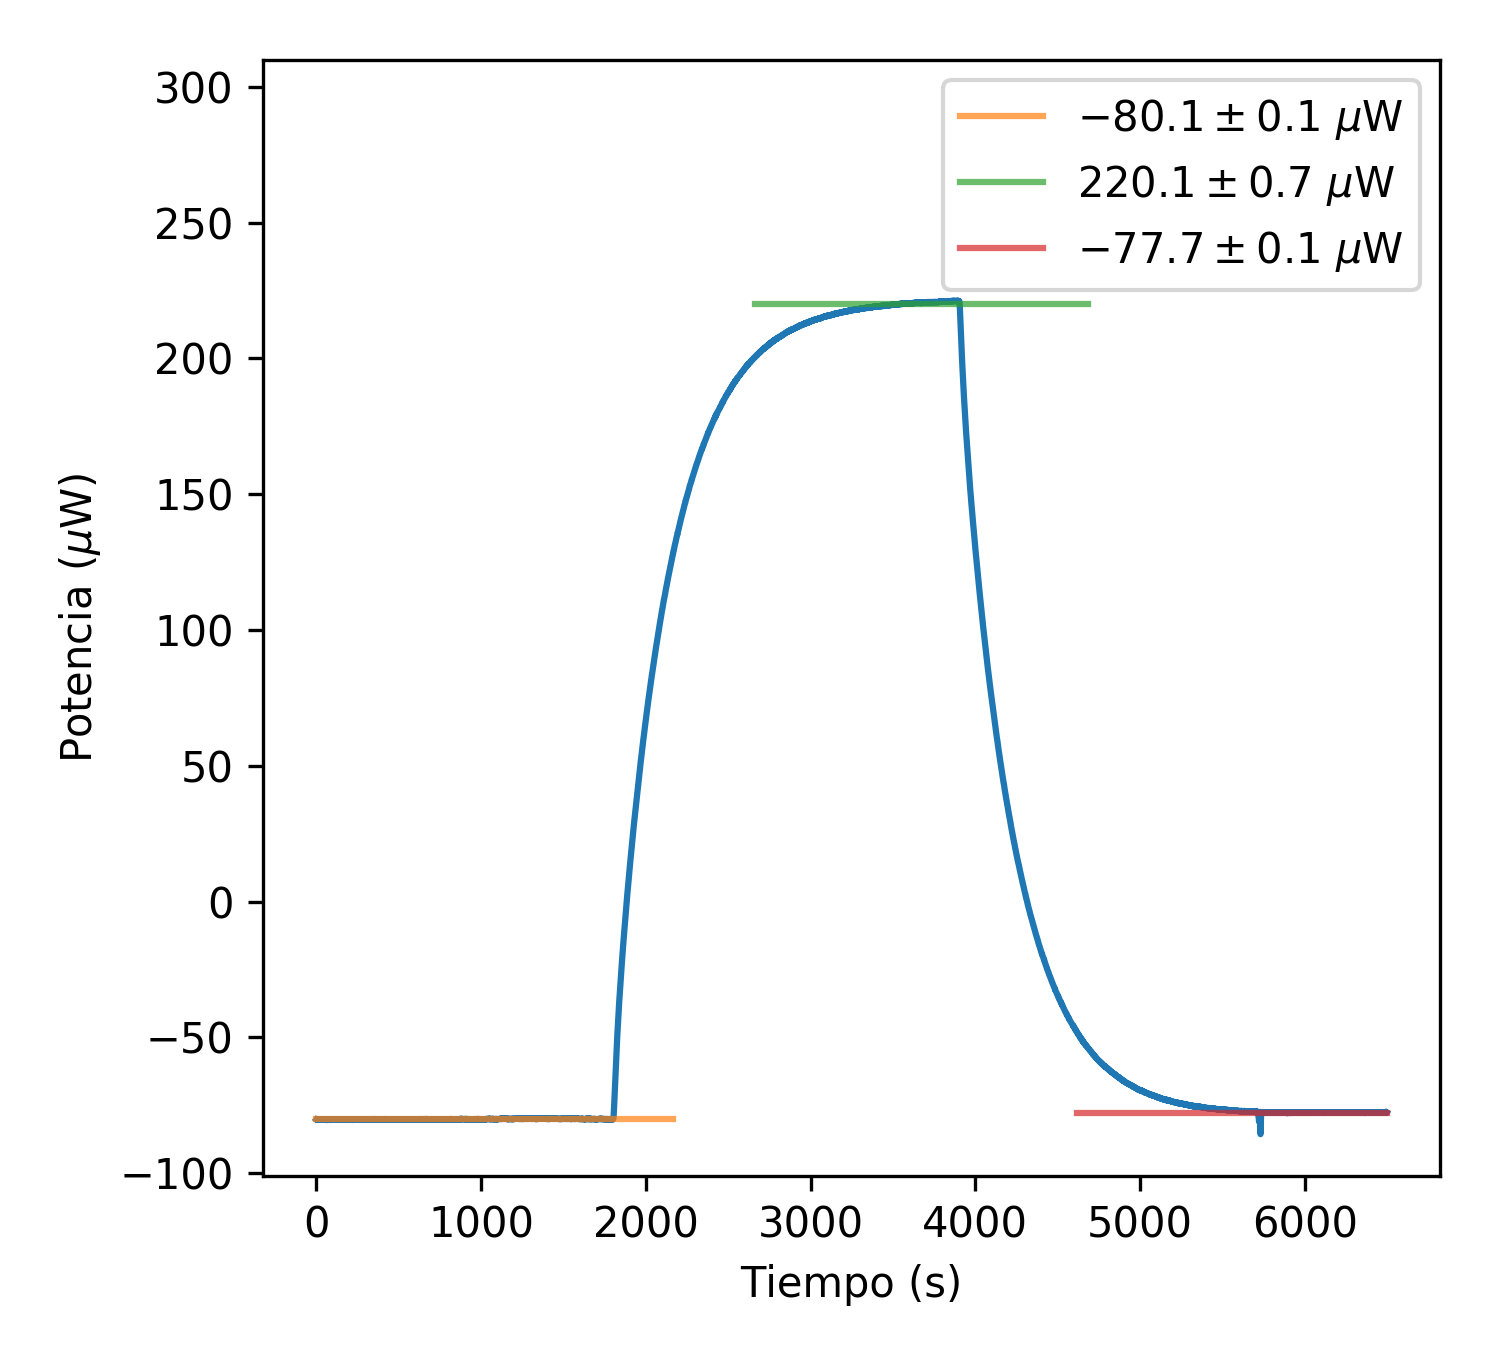
\includegraphics[width=\linewidth]{../Data/ElectricalCalibrations/Static/Calibration0}
			\caption{Potencia medida: $300.2 \pm 0.2$ $\mu$W.}
			\label{fig: noZeroCal}
		\end{subfigure}
		\caption{Ejemplos de calibraciones estáticas.}
		\label{fig: staticCalibrations}
	\end{figure}

	\newpage
	Para determinar las desviaciones a la línea base así como el valor del estado estacionario se implementó un algoritmo que se muestra en la \autoref{anx: staticCalibration} y que realiza lo siguiente:
	\begin{enumerate}
		\item Toma el valor absoluto de la derivada de la potencia.
		\item Realiza un filtro de medianas sobre los resultados anteriores, con un kernel de 101 puntos.
		\item A los puntos con valores mayores o iguales a 0,5 se les asigna un valor de 1, y los restantes 0.
		\item Se toma la derivada de los valores anteriores, de tal forma que aumentos corresponden con 1, y caídas con -1. Para el caso del estado estacionario y la última línea base, se toman el último 30 \% de los datos, en donde ya se encuentran estables estos estados. Las fronteras de estos valores determinan las fronteras de las líneas base y el estado estacionario.
		\item El promedio y desviación estándar se toma sobre cada uno de estos intervalos.
	\end{enumerate}
	
	\newpage
	\section{Din\'amica}
	En la calibración dinámica el sistema registra la línea base por 1 minuto, posteriormente aplica 40 \% de la potencia seleccionada sobre la resistencia, dando lugar a una pendiente constante por tres minutos, posteriormente, incremente nuevamente la potencia, mientras registra las pendientes observadas. Finalmente, la potencia se lleva hasta el 95 \% y se obtiene un corto estado estacionario, de esta forma el software ajusta los valores de ganancia y cero del canal \cite{Suurkuusk}. 
	\begin{figure}[h]
		\centering
		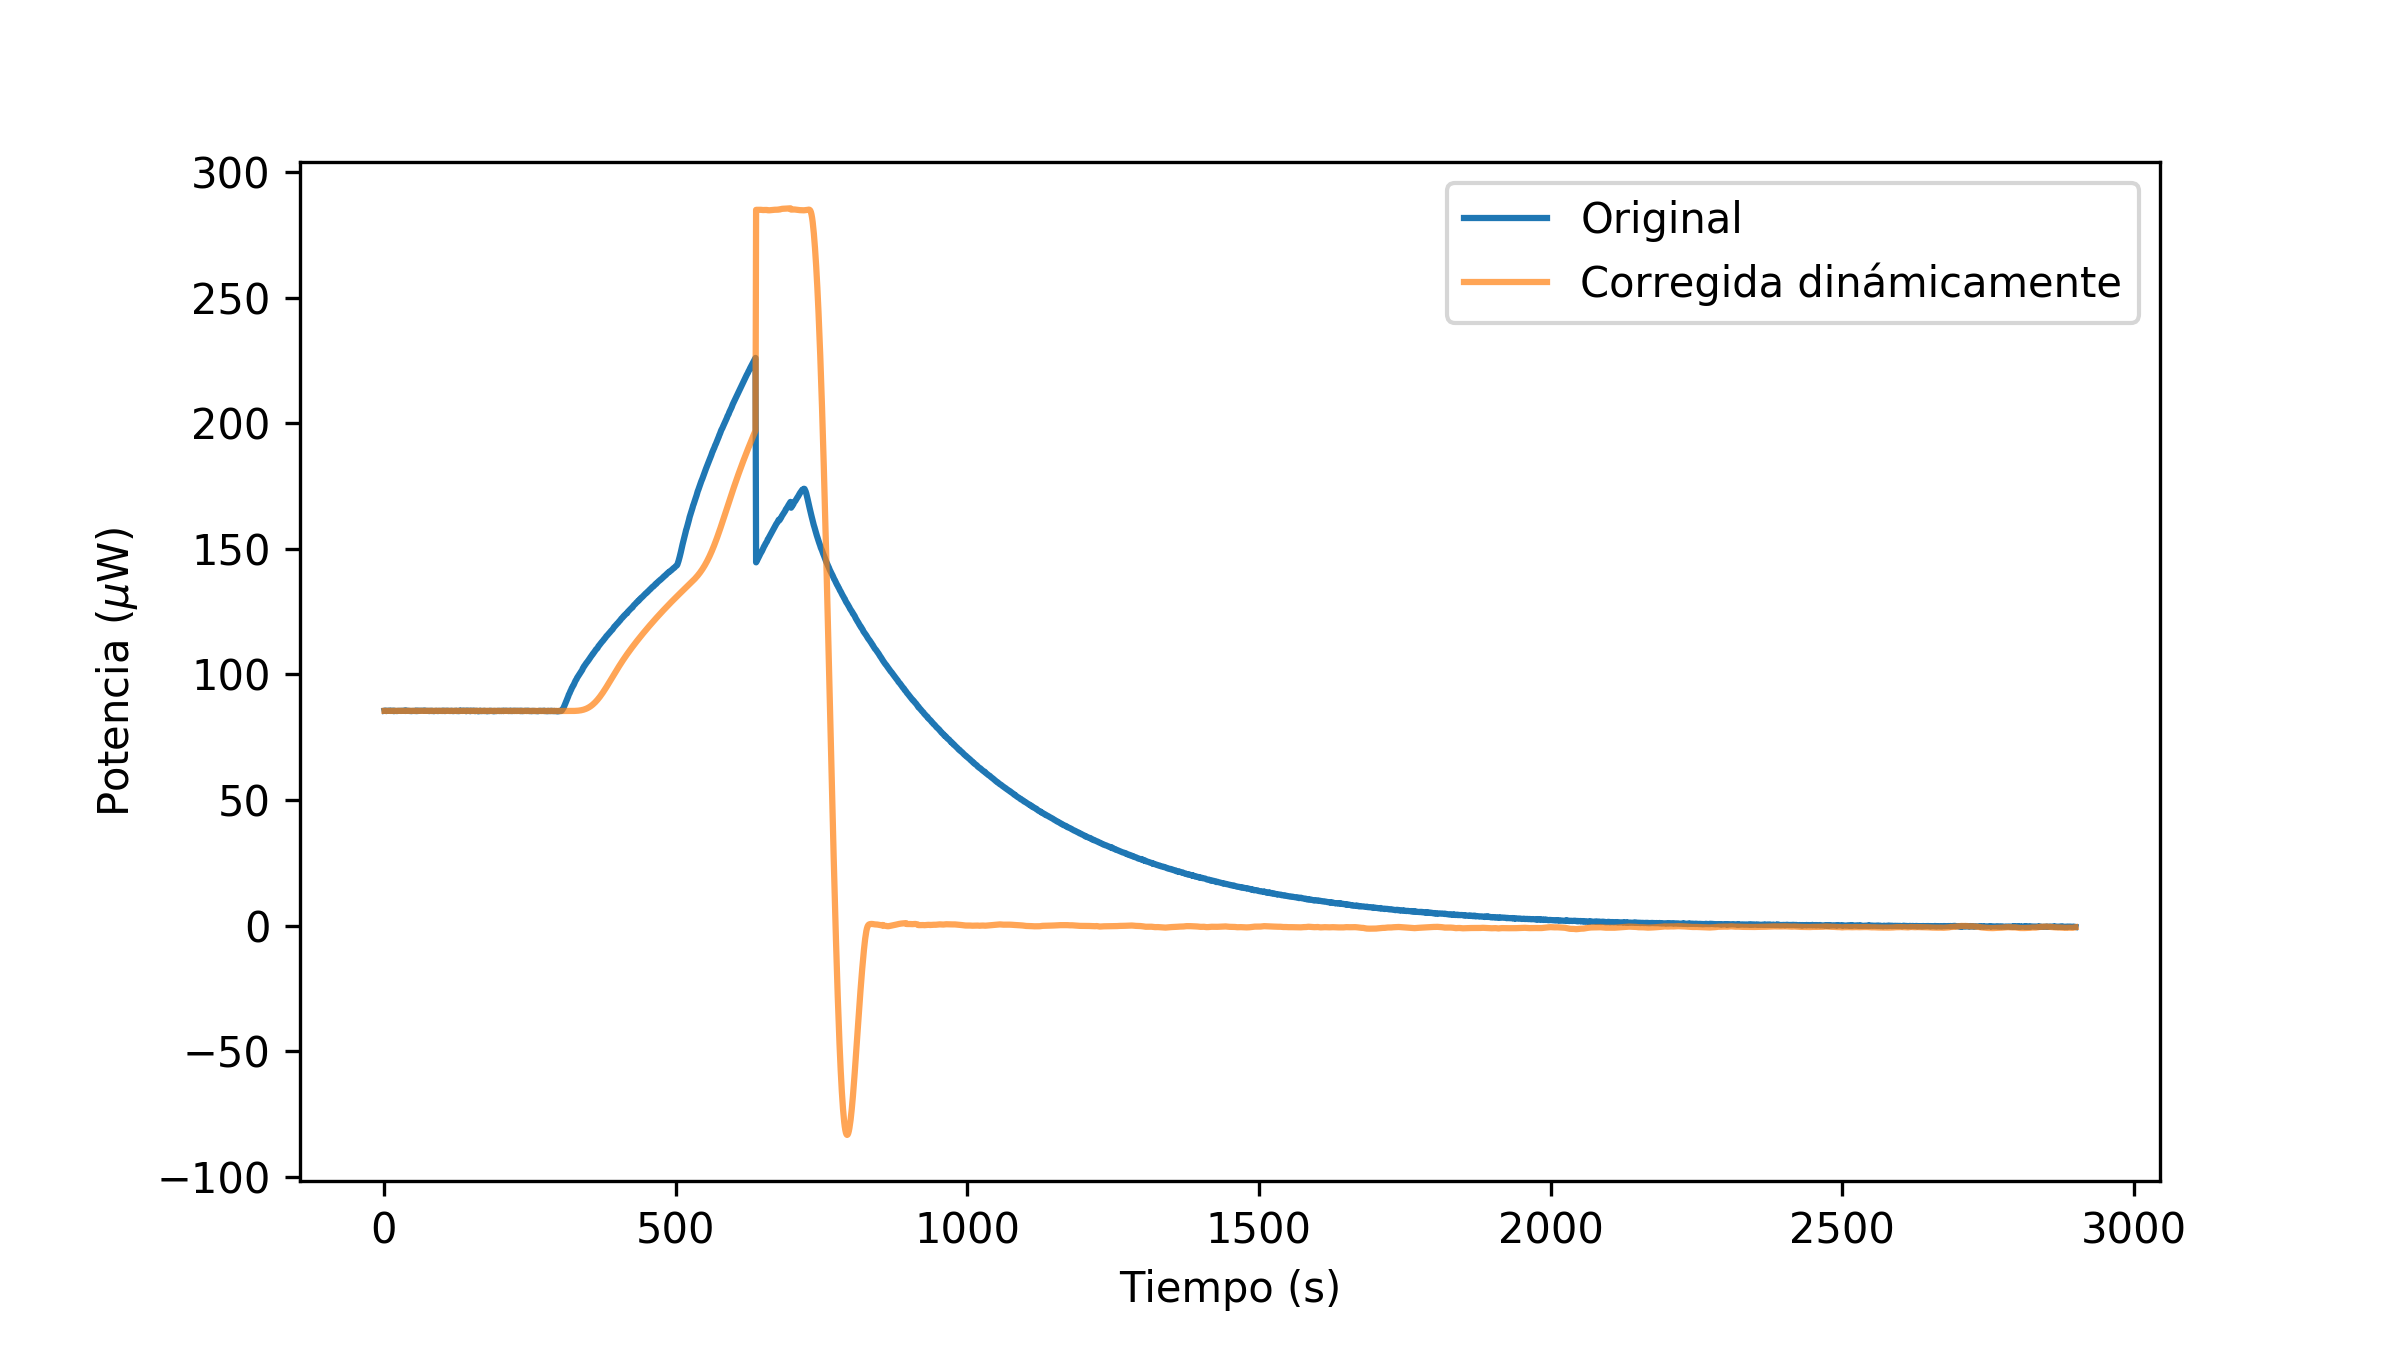
\includegraphics[width=\linewidth]{../Data/ElectricalCalibrations/Dynamic/dynamic}
		\caption{Ejemplo de una calibración dinámica.}
		\label{fig: dynamicCalibration}
	\end{figure}

	En la \autoref{fig: dynamicCalibration} se muestra un ejemplo de una calibración dinámica. En ella, la línea base se encuentra en 85,5 $\mu$W, luego de la calibración la línea base se estabiliza en -0,4 $\mu$W. La calibración dinámica permite caracterizar dos constantes que describen la inercia que presenta el calorímetro. Esto es que existe un tiempo de respuesta del equipo ante una perturbación. Luego de la calibración dinámica es posible tener una señal corregida dinámicamente, en donde se puede observar el estado estacionario al 95 \% de la potencia aplicada, y los cambios de pendiente que fueron antes mencionados.
	
	Finalmente, la calibración dinámica asegura la reproducibilidad de un experimento, como se muestra en la \autoref{fig: dynamicStatic}, en donde luego de haber realizado una calibración estática, se hace una dinámica y posteriormente para confirmar sus resultados se ejecuta una nueva calibración estática, en donde no se modifican ninguno de los parámetros en el calorímetro. En ella se observa como el inicio de las curvas de la calibración dinámica no coinciden, sin embargo, la parte final de estas se solapa, haciendo que las medidas sean reproducibles.
	\begin{figure}[h]
		\centering
		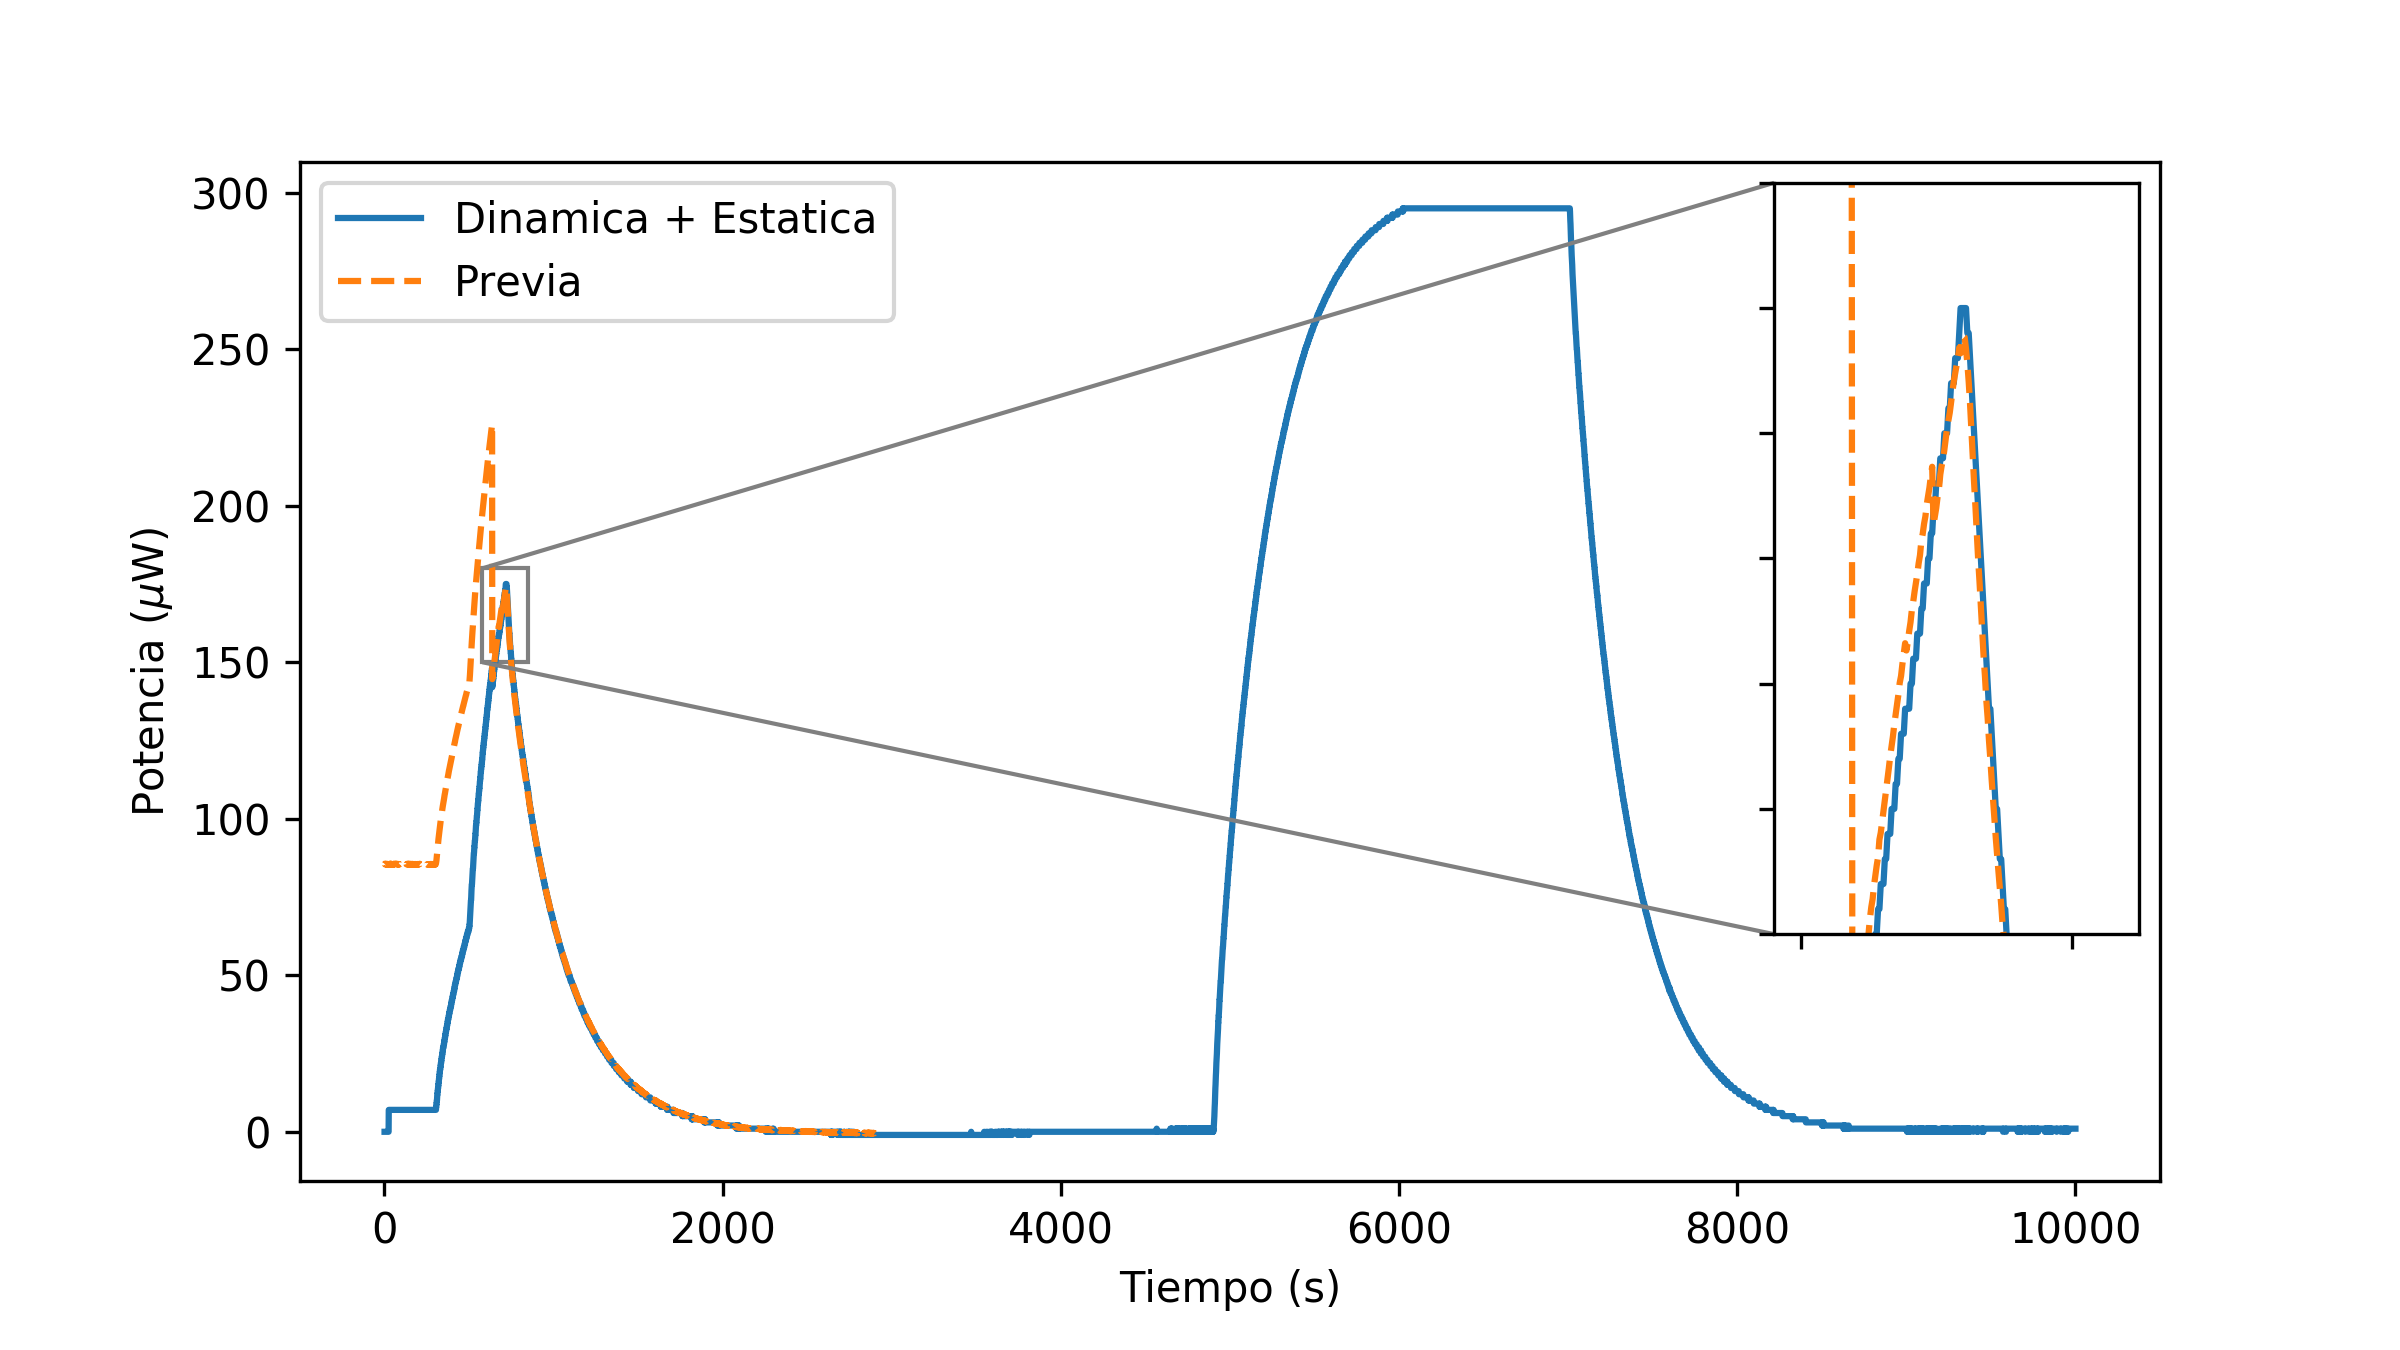
\includegraphics[width=\linewidth]{../Data/ElectricalCalibrations/Both}
		\caption{Calibraciones dinámica y estática que muestran el correcto funcionamiento del calorímetro.}
		\label{fig: dynamicStatic}
	\end{figure}
	